%%%%%%%%Bilecik �eyh Edebali �niversitesi M�hendsilik Fak�ltesi%%%%
%%%%%%%%%%%Bilgisayar M�hendisli�i Proje I-II �al��mas�%%%%%%%%%%%%
%%%%%%%%%%%%%%%%%%%%%%LaTeX Class%%%%%%%%%%%%%%%%%%%%%%%%%%%%%%%%%%
\documentclass{BUP}
\hypersetup{
    colorlinks=true,
    linkcolor=black,
    filecolor=magenta,      
    urlcolor=blue,
}
\usepackage{array}
\usepackage{subcaption}
%%%%%%%%%%%%%%%%%%%%%%%%%%%%%%%%%%%%%%%%%%%%%%%%%%%%%%%%%%%%%%%%%%%%%%%%%%%
\begin{document}
\shorthandoff{=}%grafik komutlar�nda babelden kaynaklanan hatay� engeller.
%%%%%%%%%%%%%Proje I-II �al��malar�n�n B�l�mleri%%%%%%%%%%%%%%%%%%%%%%%%%%%
\thispagestyle{empty} %Bu sayfaya sayfa numaralar� yaz�lmaz
\begin{figure}[H]
\centering

\includegraphics[scale=0.2]{logomuz}
%Bu komutla resim dosyam�z� y�kl�yoruz.
\end{figure}
%sa�a 4 sol 2 a�a�� yukar� 3%
\begin{center}
\textbf{T.C.}\\
\textbf{B�LEC�K �EYH EDEBAL� �N�VERS�TES�}\\
\textbf{M�HEND�SL�K FAK�LTES�}

\textbf{B�LG�SAYAR M�HEND�SL��� B�L�M�}
\end{center}

\vspace*{4cm}%bir miktar bo�luk b�rakmak i�in
\begin{center}
\textbf{UZAKTAN DENETLEYEB�LEN VE MESAFE �L�EN B�R ROBOT GER�EKLE�TIRMES�}

\textbf{IBRAHIM KHALIL ATTEIB YACOUB}

\textbf{Tasar�m �al��mas� I}
\end{center}

\vspace*{\fill}
\begin{center}
\textbf{Tasar�m �al��mas� I dan��man� : Prof. Dr. Cihan KARAKUZU}

\textbf{B�LEC�K}\\ 
\textbf{\today}
\end{center}

\thispagestyle{empty} %Bu sayfaya sayfa numaralar� yaz�lmaz

\begin{figure}[H]
\centering

\includegraphics[scale=0.2]{logomuz}
%Bu komutla resim dosyam�z� y�kl�yoruz.
\end{figure}
%sa� 4 sol 2 a�a�� yukar� 3%
\begin{center}
\textbf{T.C.}\\
\textbf{B�LEC�K �EYH EDEBAL� �N�VERS�TES�}\\
\textbf{M�HEND�SL�K FAK�LTES�}

\textbf{B�LG�SAYAR M�HEND�SL��� B�L�M�}
\end{center}

\vspace*{4cm}%bir miktar bo�luk b�rakmak i�in
\begin{center}
\textbf{UZAKTAN DENETLEYEB�LEN VE MESAFE �L�EN B�R ROBOT GER�EKLE�TIRMES�}

\textbf{IBRAHIM KHALIL ATTEIB YACOUB}

\textbf{Tasar�m �al��mas� I}
\end{center}

\vspace*{\fill}
\begin{center}
\textbf{Tasar�m �al��mas� I dan��man� : Prof. Dr. Cihan KARAKUZU}

\textbf{B�LEC�K}\\ 
\textbf{\today}
\end{center}

\pagenumbering{roman}%romen rakamlar� kullan�lmaya ba�lan�yor.
\setcounter{page}{2}% sayfa numaras�n� ii'den ba�lat�l�yor.
\centerline{\bf �ZET}
\addcontentsline{toc}{section}{�ZET}
\begin{center}
\textbf{Projenin Amac�}
\end{center} 
 \mbox{Bu projenin amac� Multiplo robot kullanarak uygulamalar ge�ekle�tirmesi}\\
 

\begin{center}
\textbf{Projenin Kapsam�}
\end{center}
 \mbox{Bu projenin kapsam�nda uzaktan deneteleyebilen ve mesafe �l�en bir robot ger�ekle�tirmesi }\\

\begin{center}
\textbf{Sonu�lar}
\end{center}
 \mbox{Bu projede de arac�m�z hareket halinde iken engelle kar��la�mas� an�nda istenilen mesafede}
 \mbox{durmas� sa�lanm��t�r.  �stenilen �zelliklerden biri de robotik arac�n kumanda ile kontrol edilmesi} \mbox{ger�ekle�tirilmi�tir.    }\\
%%%%%%%%%%%%%%%%%%%%%%%%%%%%%%%%%%%%%%%ABSTRACT%%%%%%%%%%%%%%%%%%%%%%%%%%%%%%%%%%%%%%%%%%
\newpage
\centerline{\bf ABSTRACT}
\addcontentsline{toc}{section}{ABSTRACT}
\begin{center}
\textbf{Project Objective}
\end{center}

 \mbox{The objective of this project is to implement applications using Multiplo robot.}\\
 
%Bilecik �eyh Edebali University Department of Computer Engineering students is studied. The aim of project is work to create a template for writing \LaTeX\ writing the final report template in the Project, to be written.

\begin{center}
\textbf{Scope of Project}
\end{center}
 \mbox{Within the scope of this project, a robot that can remotely control and measure distance has  }\\
 \mbox{been realized.}
%Bilecik �eyh Edebali University Computer Engineering Department Bilecik need to create a project template Latex codes assignment, involves the use of. The first part of the project consists of two parts, \LaTeX's development have been studied and why it is preferred that the use of information provided in the information. Faculty of Engineering of the university for the second part, Sheikh Edebali Bilecik Project Paper \LaTeX\ codes and are included.

\begin{center}
\textbf{Results}
\end{center}
 \mbox{In this project, while our vehicle is in motion, it is ensured that it stops at the desired distance }\\
  \mbox{when it encounters an obstacle. One of the desired features is the control of the robotic vehicle}
  \mbox{with the remote control.}
%As a result, Bilecik Sheikh Edebali University Computer Engineering
%Department prepared a document that students can build project reports into \LaTeX. 
\addcontentsline{toc}{section}{TE�EKK�R}
\section*{TE�EKK�R}
Bu projenin ba��ndan sonuna kadar haz�rlanmas�nda  eme�i bulunan ve 
beni bu konuya y�nlendiren sayg�de�er hocam ve dan��man�m 
Say�n Prof. Dr. Cihan KARAKUZU'a t�m katk�lar�ndan ve hi� 
eksiltmedi�i deste�inden dolay� te�ekk�r ederim.
\vspace{2cm}

\begin{flushright}
\textbf{IBRAHIM KHALIL ATTEIB YACOUB}

\today
\end{flushright}
\tableofcontents%bu komutun oldu�u yerde i�indekiler olu�turulur.
%\textbf{\centerline{\bf S�MGE L�STES�}}
\addcontentsline{toc}{section}{S�MGE L�STES�}

\renewcommand*\listfigurename{\centerline{\bf\normalsize �EK�L L�STES�}}
\listoffigures%bu komutun oldu�u yerde �ekiller listesi olu�turulur
\addcontentsline{toc}{section}{�EK�L L�STES�}
\renewcommand*\listtablename{\centerline{\bf\normalsize TABLO L�STES�}}
\listoftables%bu komutun oldu�u yerde tablolar listesi olu�turulur
\addcontentsline{toc}{section}{TABLO L�STES�}
\pagenumbering{arabic}%Sayfa numaralamas�n� arap rakamlar�yla yapar.
\setcounter{page}{1}%sayfa numaras�n� 1'den ba�lat�r.
\section{G�R��}
Bir robot in�a etmek, ba�ka bir �ey in�a etmek gibidir. Sadece bir fikriniz olmas� gerekiyor
hayal g�c�n�zden ve onu in�a etme cesaretinizden. Ve tabii ki sab�r. Ama i�ler �ok
standart bir yap�m y�nteminiz yoksa daha zor. Bu y�zden Multiplo'yu geli�tiriyoruz
farkl� disiplinlerin bir entegrasyonu olarak, b�ylece hi�bir zorluk �ekmezsiniz.
mekanik veya elektronik ile. Ve b�ylece, yaratma s�recine odaklanabilirsiniz.

bu konseptten yola ��karak bu projede iki uygulamay� ger�ekle�tirmeye �al��aca��z.
Bu uygulamalar ��rencilerin temel bir robotik kavram�na sahip olmalar�n� sa�lar.

�lk uygulamam�za \textbf{Kumanda ile hareket ettirmek}, ikinci ise \textbf{Engel alg�lmak}.\\
�al��malar�m�z� basit a��klamalar, algoritmalar ve ad�m ad�m g�steren resimlerle destekleyece�iz, b�ylece kolay ve anla��l�r olacakt�r.
\section{KULLANILAN ROBOT VE PROGRAM}
Bu b�l�mde proje geli�tirme a�amas�nda kullan�lan robot ve ve program bahsedilmi�tir.
\subsection{Multiplo}
Multiplo, kullan�c�lar�n y�ksek teknolojili cihazlar tasarlamalar�n� ve olu�turmalar�n� sa�layan a��k kaynakl� bir felsefeye dayanan bir robotik bina sistemidir. �u anda okullar ve robotik merakl�lar� taraf�ndan ��retim materyali olarak kullan�lmaktad�r.

Multiplo platformlarda d�zenlenmi�tir. Platform, yayg�n robotik sorunlar� ��zmek ve ��zmek i�in olu�turulan bir sistem mod�lleri k�mesidir.

�ekil \ref{fig:multi_robot}'de Mutliplo ara� kiti �rne�idir.
\begin{figure}[h!]
\centering
  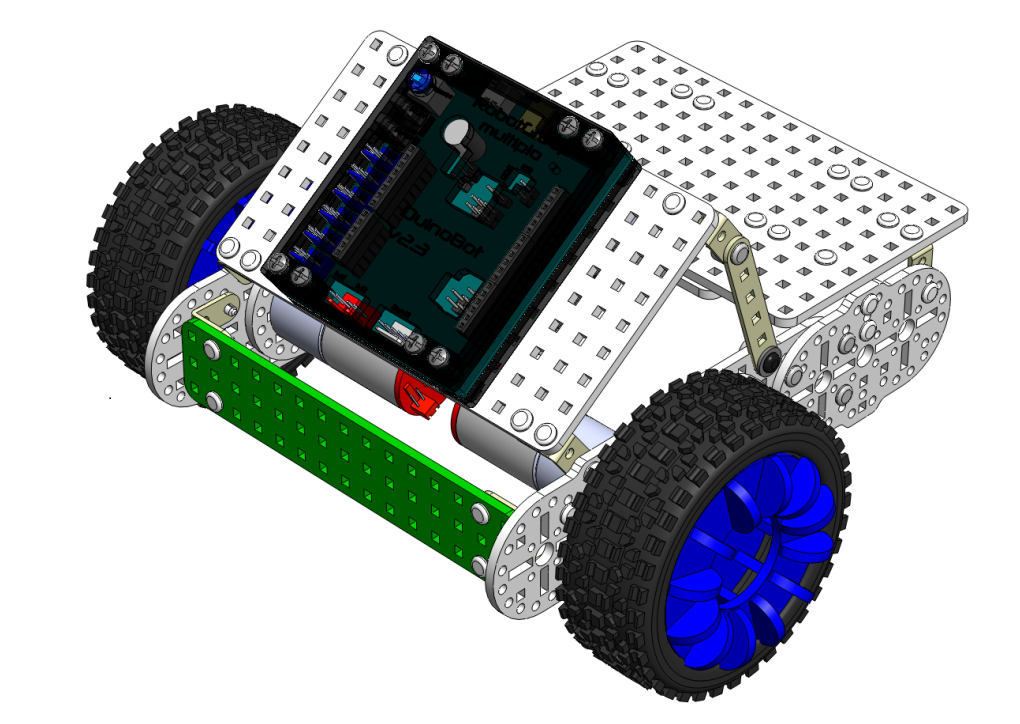
\includegraphics[scale=0.4]{robot.png}
  \caption{Multiplo ara� kiti}
  \label{fig:multi_robot}
\end{figure}

\textbf{Elektronik}: Arduino ile uyumlu\\
\textbf{Yaz�l�m}: Arduino'nun yan� s�ra, A��k Kaynak grafik IDE miniBloq ile uyumludur\\
\textbf{Mekanik}: ABS, akrilik ve fablabuyumlu olarak kolayca �zelle�tirilebilir di�er malzemelere dayal�\\
\textbf{Belgeler}: LibreOffice gibi A��k Kaynak bi�imlerinde yay�mlan�r\\


Multiplo robotlar Kaliforniya'da Teknoloji M�zesi'nde sergileniyor.  Konsepti ba�lang��ta Julian da Silva ve baz� i�birlik�ileri taraf�ndan tasarlanm��t�r, daha sonra �irket taraf�ndan benimsenmi�tir. Rodolfo Cossovich taraf�ndan bir robot kitine d�n��t�r�ld�kten sonra nihayet kitlesel fonlama kampanyas�yla kitlesel fonlama yap�ld�.\cite{multiplo}


\subsection{miniBloq}
MiniBloq, Arduino, Multiplo, fiziksel bilgi i�lem cihazlar� ve robotlar i�in grafiksel bir programlama ortam�d�r. 

Temel hedeflerinden biri, o�renciler ve yeni ba�layanlara fiziksel bilgi i�lem ve robotik platformlar� daha da yak�nla�t�rmakt�r.\cite{miniBloq}

miniBloq �zellikleri Tablo \ref{table:1}'de verilmi�tir.
\begin{table}[h!]
\centering
\begin{tabular}{|c| m{20em}|} 
\hline
 �zellik & A��klama\\
\hline
 Kolay & Sadece birka� t�klama ve ilk program�n�z �al���yor. \\
\hline
Ger�ek zamanl� kod olu�turucu & Kodu, s�zdizimi renkli bir pencerede g�steren bloklar eklerken veya param de�erlerini de�i�tirirken olu�turur.\\
\hline
Ger�ek zamanl� hata denetimi &\\
\hline
Otomatik bo�luklu temel s�r�kle ve b�rak &\\
\hline
Geli�mi� arabirim & Yak�nla�t�rma, kesme ve yap��t�rma, sabitlenebilir pencereler ve klavye gezintisi miniBloq GUI'nin �zelliklerinden sadece baz�lar�d�r.\\
\hline
G�m�l� terminal & Seri/USB ba�lant� noktalar� �zerinden panonuza veri g�ndermenizi ve alman�z� sa�layan g�m�l� bir terminal vard�r\\
\hline
Hepsi bire bir kullan�ma haz�r ��z�m & Paket �al��maya ba�lamak i�in her �eyi i�erir\\
\hline
Mod�ler ve geni�letilebilir & Kullan�c� kolayca kendi yeni bloklar�n� olu�turabilir\\
\hline
\end{tabular}
\caption{miniBloq �zellikleri}
\label{table:1}
\end{table}
\newpage
miniBloq ilk a�t���n�zda �ekil \ref{fig:minibloq}'de gibi kar��n�zda bir ekran ��kacakt�r.
\begin{figure}[h!]
  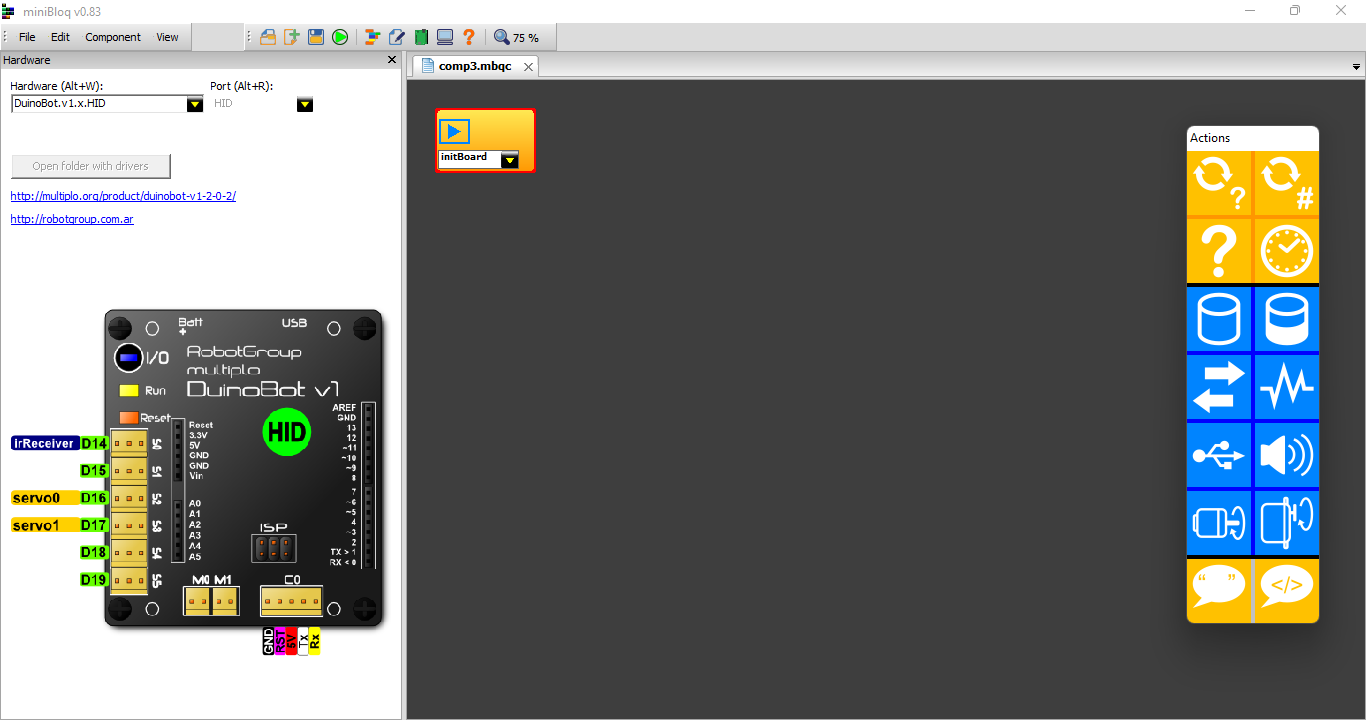
\includegraphics[scale=0.4]{minibloq.png}
  \caption{miniBloq giri� ekran�}
  \label{fig:minibloq}
\end{figure}
\section{PROJEN�N TASARIMI VE �ALI�MA YAPISI}
Bu b�l�mde projenin tasar�m� ve �al��sma yap�s�ndan bahsedilmektedir
\subsection{Projenin Tasar�m�}
Bu projede iki arka tekerle�i ve bir �nde birer tekerle�i olan bir Multiplo robotu kullanaca��z. Bu robotun montaj� hakk�nda daha fazla bilgi i�in ayri bir dok�man haz�rlad�k, dok�mana g�rmek i�in \href{https://drive.google.com/file/d/11VlHap81XU32XOVKXIDdKzzte7GgiFI3/view?usp=sharing}{buraya tiklay�n}

\begin{figure}[h!]
\centering
  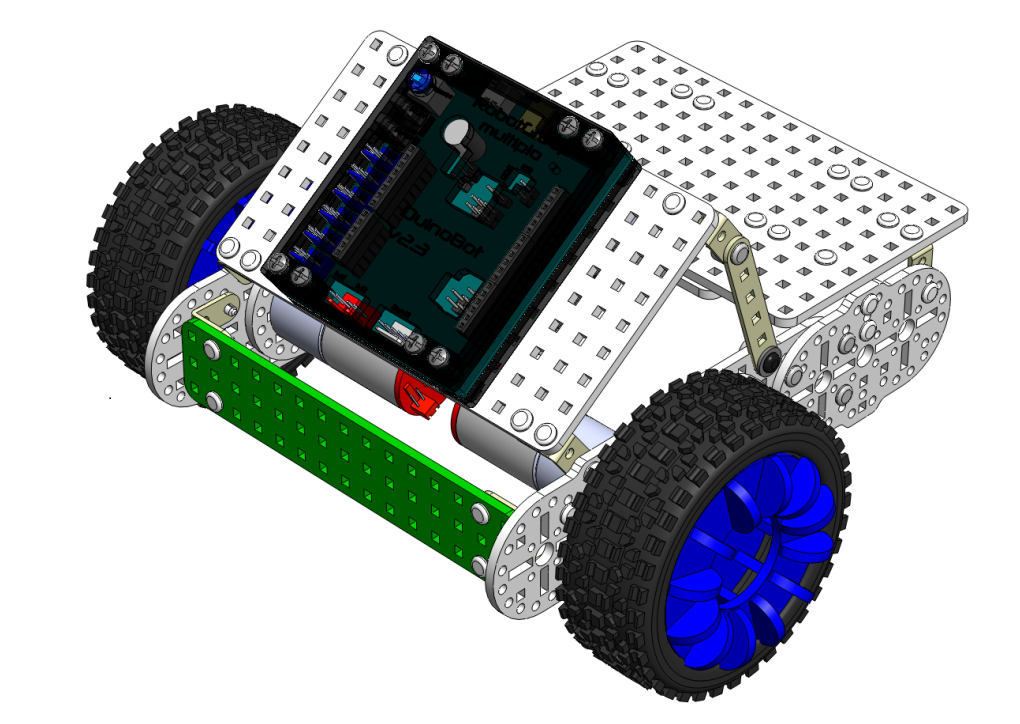
\includegraphics[scale=0.5]{robot.png}
  \caption{Projede kulland���m�z robot}
  \label{fig:robot}
\end{figure}

Giri�te size s�yledi�imiz gibi, bu proje iki uygulamay� ger�ekle�tirmeye ama�l�d�r
\begin{itemize}
\item Kumanda ile hareket ettirmek
\item Engel Alg�lama
\end{itemize}

olup projenin �al��ma yap�s� k�sm�nda bu uygulamalar ile ilgili detayl� bilgiler verilmi�tir.

\subsection{Projenin �al��ma Yap�s�}
Bu b�l�mde projenin �al��ma yap�s�ndan bahsedilmektedir.
\subsubsection{Kumanda ile hareket ettirme}
Programlama a�amas�na ge�meden �nce ad�mlar� \label{fig:kumanda} bir ak�� diyagram� ile a��klamaya �al���yoruz.
\begin{figure}[h!]
\centering
  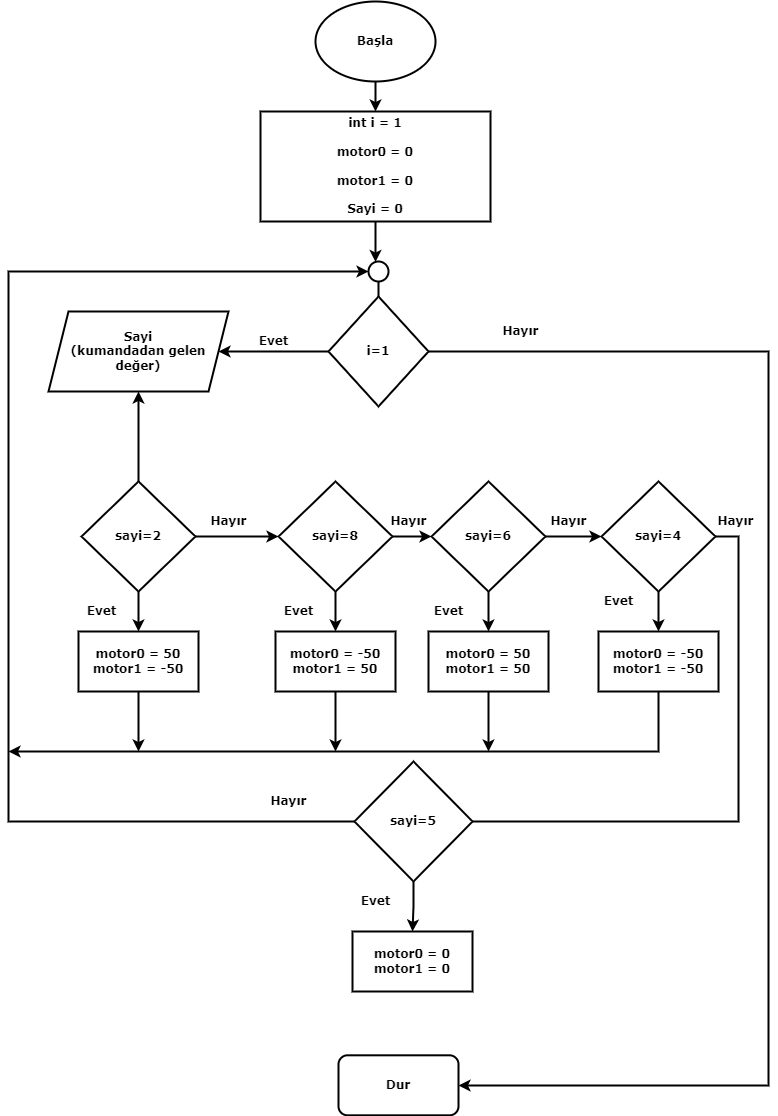
\includegraphics[scale=0.4]{kumanda.png}
  \caption{Kumanda ile hareket ettirme ak�� diyagram�}
  \label{fig:kumanda}
\end{figure}

Ak�� diyagram�m�z� �izdikten sonra programlama a�amas�na ge�iyoruz.

�nce miniBloq olan program�m�z� a��yoruz, ard�ndan k�rm�z� renk ile �izdi�imiz sembol� se�iyoruz, bu sembol bir de�i�keni ifade ediyor. De�i�kenimize isim olarak "speed" atad�k. �imdi daire i�ine ald���m�z k�sma t�kl�yoruz, k�rm�z� ile �izdi�imiz de�eri belirten \# sembol�n� se�memizi sa�layan bir pencere a��l�yor. "speed" de�i�kenimize 50 de�eri veriyoruz ve de�er olarak s�f�ra "code" adl� ba�ka bir de�i�ken ekliyoruz yani 2 de�i�kenimiz var.\\
speed=50
code = 0
\begin{figure}[h!]
     \centering
     \begin{subfigure}[b]{0.3\textwidth}
         \centering
         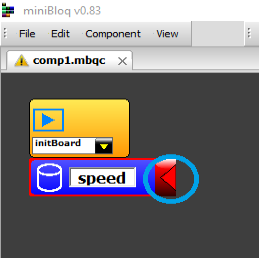
\includegraphics[width=\textwidth]{val_1}
         \caption{}
         \label{fig:val_1}
     \end{subfigure}
     \hfill
     \begin{subfigure}[b]{0.3\textwidth}
         \centering
         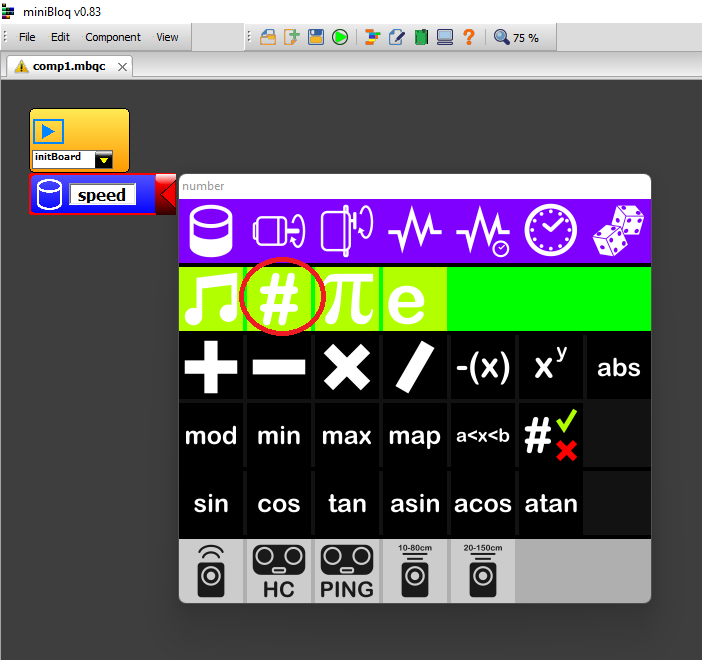
\includegraphics[width=\textwidth]{val_2}
         \caption{}
         \label{fig:val_2}
     \end{subfigure}
     \hfill
     \begin{subfigure}[b]{0.3\textwidth}
         \centering
         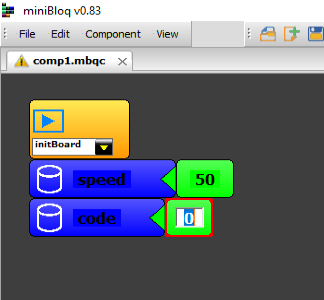
\includegraphics[width=\textwidth]{val_3}
         \caption{}
         \label{fig:val_3}
     \end{subfigure}
        \caption{miniBloq de�i�ken tan�mla}
        \label{fig:miniBloq degisken tanimla}
\end{figure}

De�i�kenlerimizi ald�ktan sonra bir d�ng� ihtiyac�m�z var. Program� hep �al���r durumda b�rakmak istiyoruz. �imdi bunu while d�ng�s�yle nas�l yapabilece�imizi a��kl�yoruz.
\begin{figure}[h!]
     \centering
     \begin{subfigure}[b]{0.23\textwidth}
         \centering
         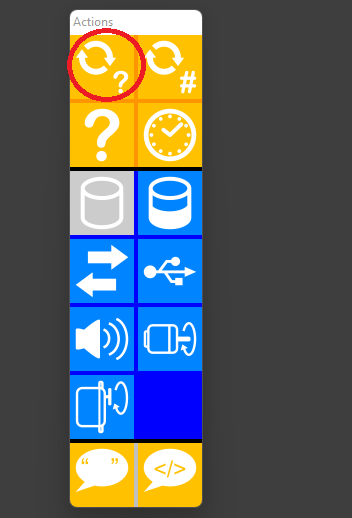
\includegraphics[width=\textwidth]{while_1}
         \caption{}
         \label{fig:while_1}
     \end{subfigure}
     \hfill
     \begin{subfigure}[b]{0.23\textwidth}
         \centering
         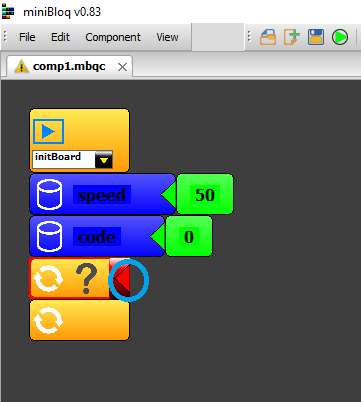
\includegraphics[width=\textwidth]{while_2}
         \caption{}
         \label{fig:while_2}
     \end{subfigure}
     \hfill
     \begin{subfigure}[b]{0.23\textwidth}
         \centering
         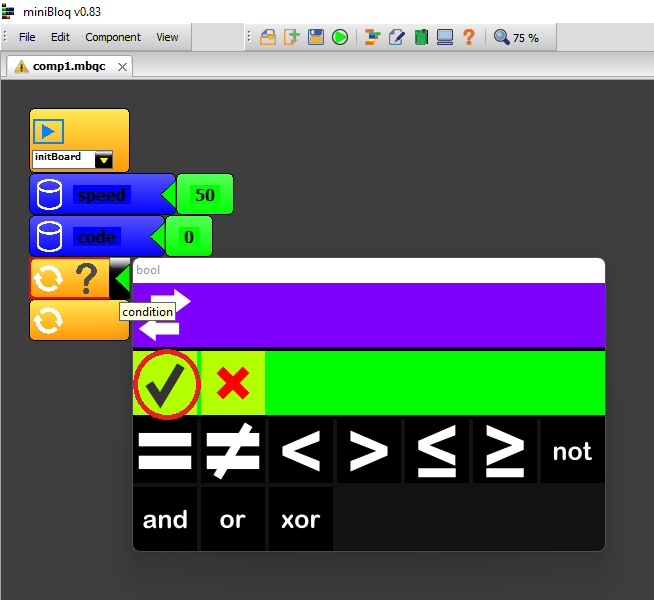
\includegraphics[width=\textwidth]{while_3}
         \caption{}
         \label{fig:while_3}
     \end{subfigure}
         \hfill
     \begin{subfigure}[b]{0.23\textwidth}
         \centering
         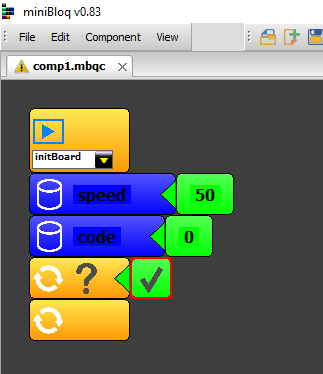
\includegraphics[width=\textwidth]{while_4}
         \caption{}
         \label{fig:while_4}
     \end{subfigure}
        \caption{While D�ng�s� tan�mlama a�amalar�}
        \label{fig:while_dongusu}
\end{figure}
\newpage
Daha sonra uzaktan kumandadan gelen de�ere ihtiyac�m�z var, bunu yapabilmek i�in kumandadan gelen de�eri code de�i�kenimize atamam�z gerekiyor.
\begin{figure}[h!]
     \centering
     \begin{subfigure}[b]{0.3\textwidth}
         \centering
         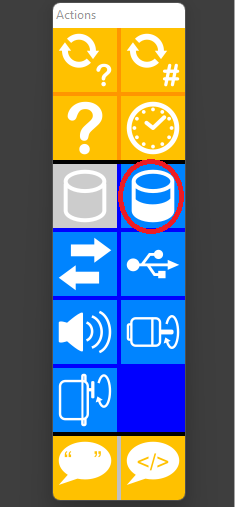
\includegraphics[width=\textwidth]{ata_1}
         \caption{}
         \label{fig:ata_1}
     \end{subfigure}
     \hfill
     \begin{subfigure}[b]{0.3\textwidth}
         \centering
         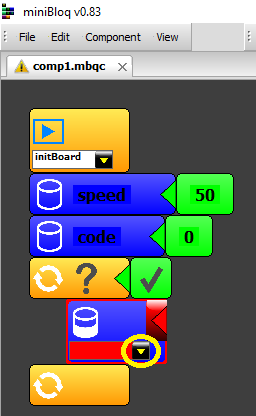
\includegraphics[width=\textwidth]{ata_2}
         \caption{}
         \label{fig:ata_2}
     \end{subfigure}
     \hfill
     \begin{subfigure}[b]{0.3\textwidth}
         \centering
         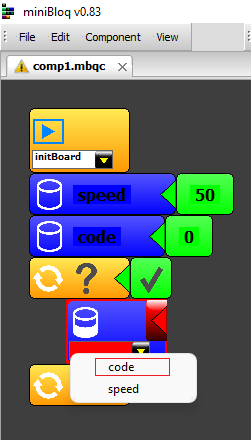
\includegraphics[width=\textwidth]{ata_3}
         \caption{}
         \label{fig:ata_3}
     \end{subfigure}
         \hfill
     \begin{subfigure}[b]{0.3\textwidth}
         \centering
         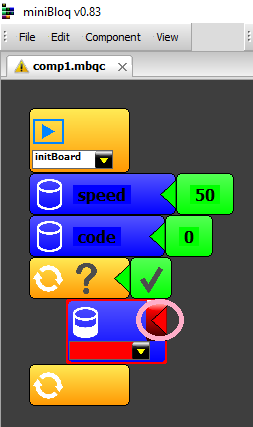
\includegraphics[width=\textwidth]{ata_4}
         \caption{}
         \label{fig:ata_4}
     \end{subfigure}
      \hfill
     \begin{subfigure}[b]{0.3\textwidth}
         \centering
         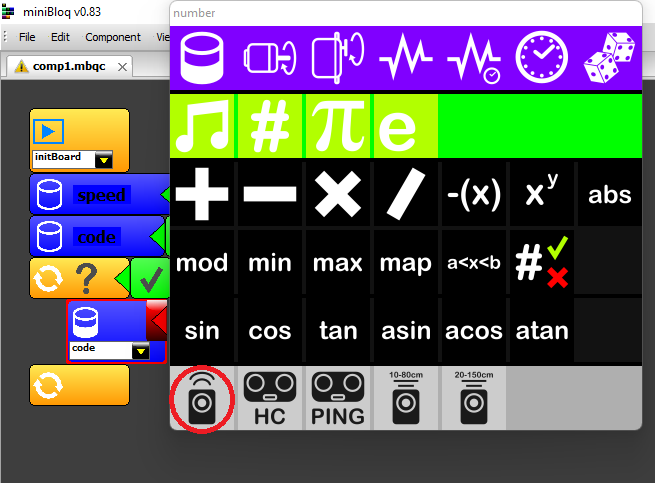
\includegraphics[width=\textwidth]{ata_5}
         \caption{}
         \label{fig:ata_5}
     \end{subfigure}
      \hfill
     \begin{subfigure}[b]{0.3\textwidth}
         \centering
         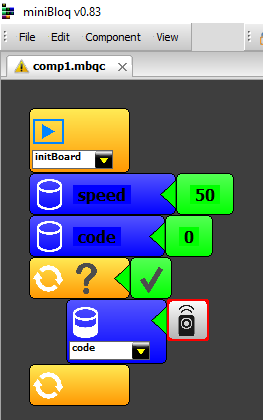
\includegraphics[width=\textwidth]{ata_6}
         \caption{}
         \label{fig:ata_6}
     \end{subfigure}
        \caption{De�i�keni de�er atma i�lemler}
        \label{fig:degisken_val}
\end{figure}
\newpage
Uzaktan kumandadan gelen de�eri alabildik. �imdi gelen de�erleri kontrol edebilmek i�in ko�ullar� ayarlayaca��z ve buna g�re robotumuzun hareketlerini y�netece�iz.\\
ilk ko�ul gelen say�n�n 2 olup olmad���n� kontrol etmektir.
\begin{figure}[h!]
     \centering
     \begin{subfigure}[b]{0.23\textwidth}
         \centering
         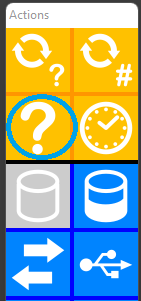
\includegraphics[width=\textwidth]{if_1}
         \caption{}
         \label{fig:if_1}
     \end{subfigure}
     \hfill
     \begin{subfigure}[b]{0.23\textwidth}
         \centering
         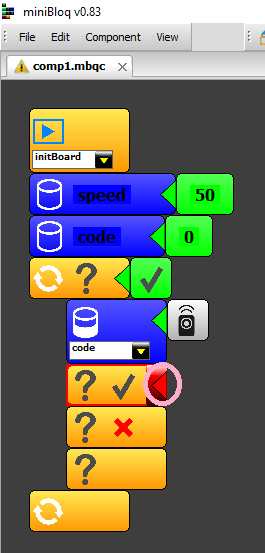
\includegraphics[width=\textwidth]{if_2}
         \caption{}
         \label{fig:if_2}
     \end{subfigure}
     \hfill
     \begin{subfigure}[b]{0.23\textwidth}
         \centering
         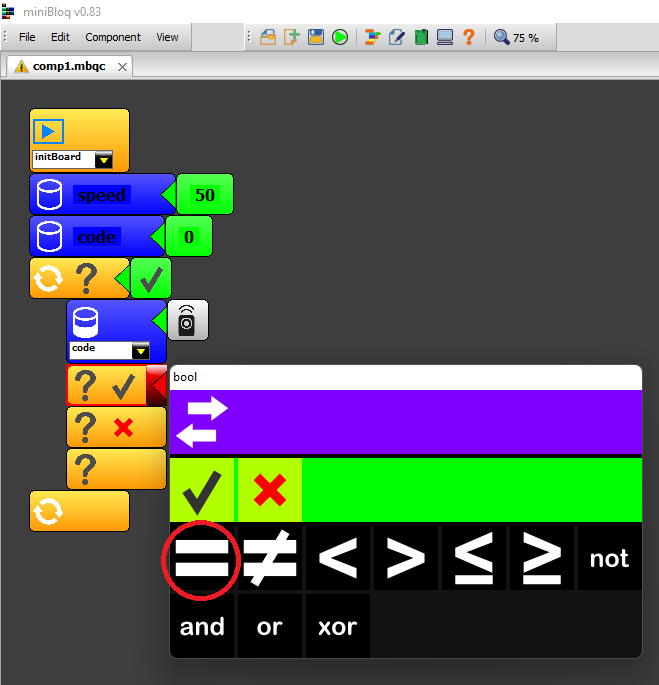
\includegraphics[width=\textwidth]{if_3}
         \caption{}
         \label{fig:if_3}
     \end{subfigure}
         \hfill
     \begin{subfigure}[b]{0.23\textwidth}
         \centering
         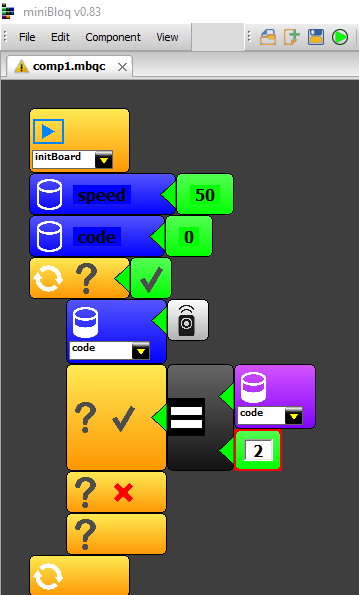
\includegraphics[width=\textwidth]{if_4}
         \caption{}
         \label{fig:if_4}
     \end{subfigure}
        \caption{Birinci ko�ul kumandadan gelen de�er 2 ise}
        \label{fig:kumanda_value_2}
\end{figure}

Gelen say�n�n de�erinin 2 oldu�unu varsayal�m, o zaman robotu 50 h�zla ilerletece�iz\\
Bunu yapmak i�in motor0'a 50 ve motor1'e -50 atad�k

\begin{figure}[h!]
     \centering
     \begin{subfigure}[b]{0.17\textwidth}
         \centering
         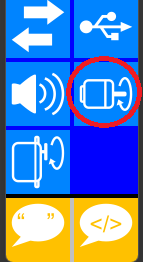
\includegraphics[width=\textwidth]{motor_1}
         \caption{}
         \label{fig:motor_1}
     \end{subfigure}
     \hfill
     \begin{subfigure}[b]{0.17\textwidth}
         \centering
         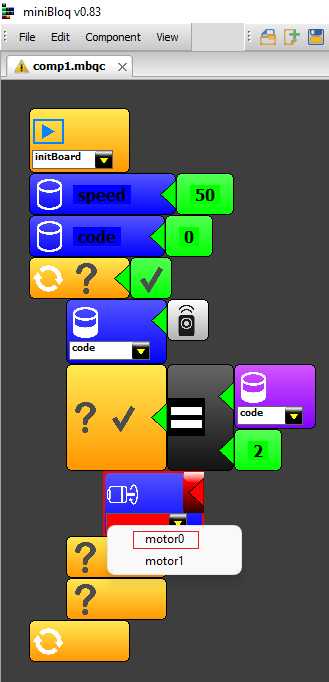
\includegraphics[width=\textwidth]{motor_2}
         \caption{}
         \label{fig:motor_2}
     \end{subfigure}
     \hfill
     \begin{subfigure}[b]{0.17\textwidth}
         \centering
         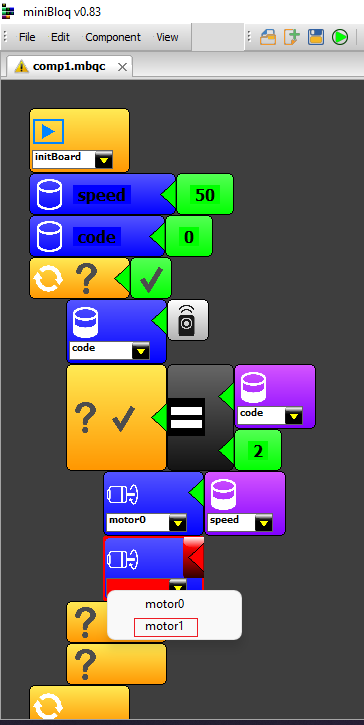
\includegraphics[width=\textwidth]{motor_3}
         \caption{}
         \label{fig:motor_3}
     \end{subfigure}
         \hfill
     \begin{subfigure}[b]{0.17\textwidth}
         \centering
         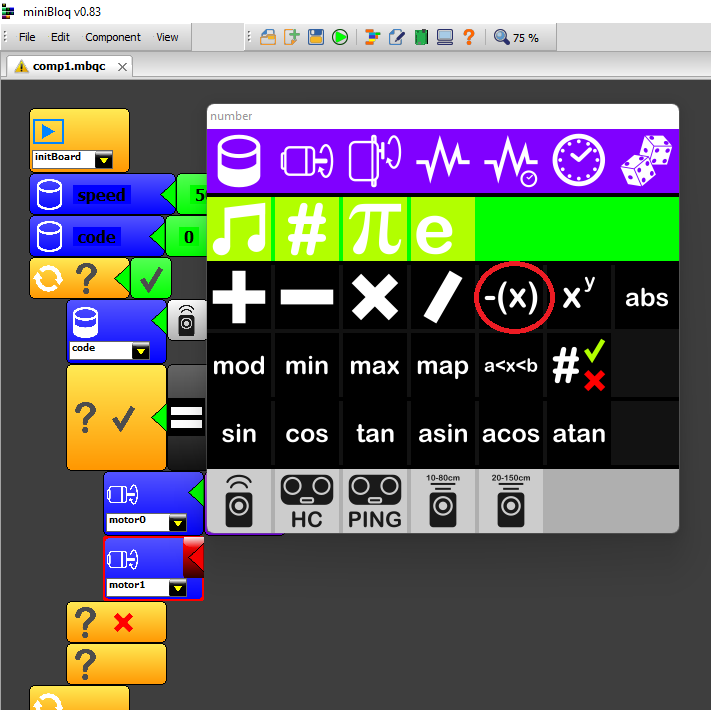
\includegraphics[width=\textwidth]{motor_4}
         \caption{}
         \label{fig:motor_4}
     \end{subfigure}
      \hfill
     \begin{subfigure}[b]{0.17\textwidth}
         \centering
         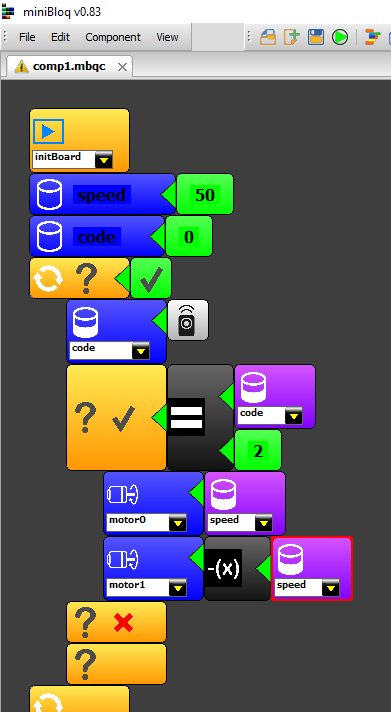
\includegraphics[width=\textwidth]{motor_5}
         \caption{}
         \label{fig:motor_5}
     \end{subfigure}
        \caption{�leriye do�ru}
        \label{fig:devant}
\end{figure}
\newpage
Kumandadan gelen de�er 8 ise motor0 -50 ve motor1 50 atayarak robotumuz geriye gidiyor
\begin{figure}[h!]
\centering
  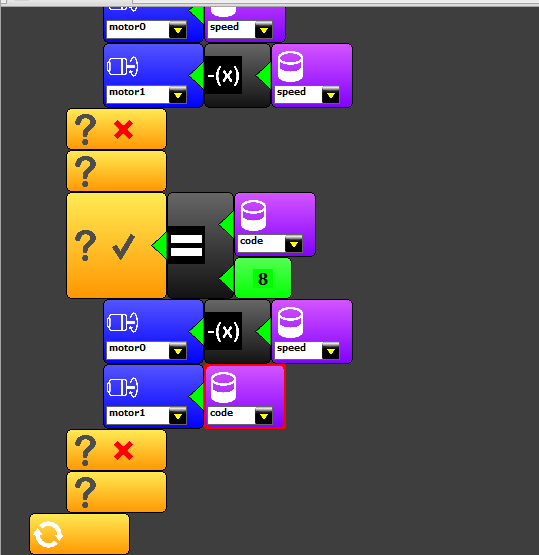
\includegraphics[width=0.6\textwidth]{code_8.png}
  \caption{Geriye do�ru }
  \label{fig:code_8}
\end{figure}

Robotun sa�a d�nmesini sa�lamak i�in her iki motora da 50 h�z atamam�z yeterlidir.\\
bu i�lemi ger�ekle�tirmek i�in uzaktan kumandaya 6 de�erini veriyoruz
\begin{figure}[h!]
\centering
  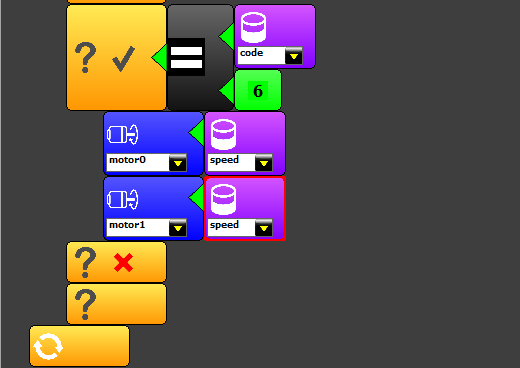
\includegraphics[width=0.7\textwidth]{code_6.png}
  \caption{Sa�a d�n}
  \label{fig:code_6}
\end{figure}

Tabii sa�a d�nebiliyorsa sola da d�nebilir, peki bunu nas�l yapaca��z? \\
Basit bir �ekilde her iki motora da -50 atayarak ger�ekle�tirebiliriz.\\
bu i�lem i�in 4 de�erini verebiliriz
\begin{figure}[h!]
\centering
  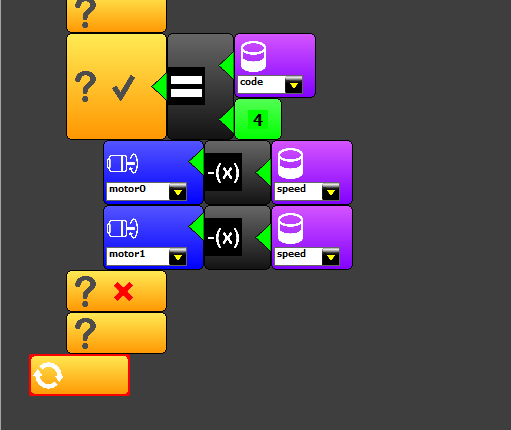
\includegraphics[width=0.6\textwidth]{code_4.png}
  \caption{Sola d�n}
  \label{fig:code_4}
\end{figure}

Robotu istedi�imiz y�ne y�nlendirebildik, �imdi 5 tu�una bast���m�zda durmas�n� istiyoruz.
\begin{figure}[h!]
\centering
  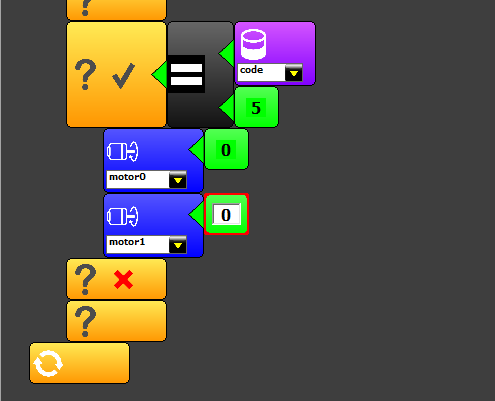
\includegraphics[width=0.6\textwidth]{code_5.png}
  \caption{Reset atma}
  \label{fig:code_5}
\end{figure}

\newpage
�lk uygulaman�z bitti, size uygulama s�ras�nda kulland���m�z malzemelerin bir tablosunu yapaca��z.
\begin{figure}[h!]
     \centering
     \begin{subfigure}[b]{0.2\textwidth}
         \centering
         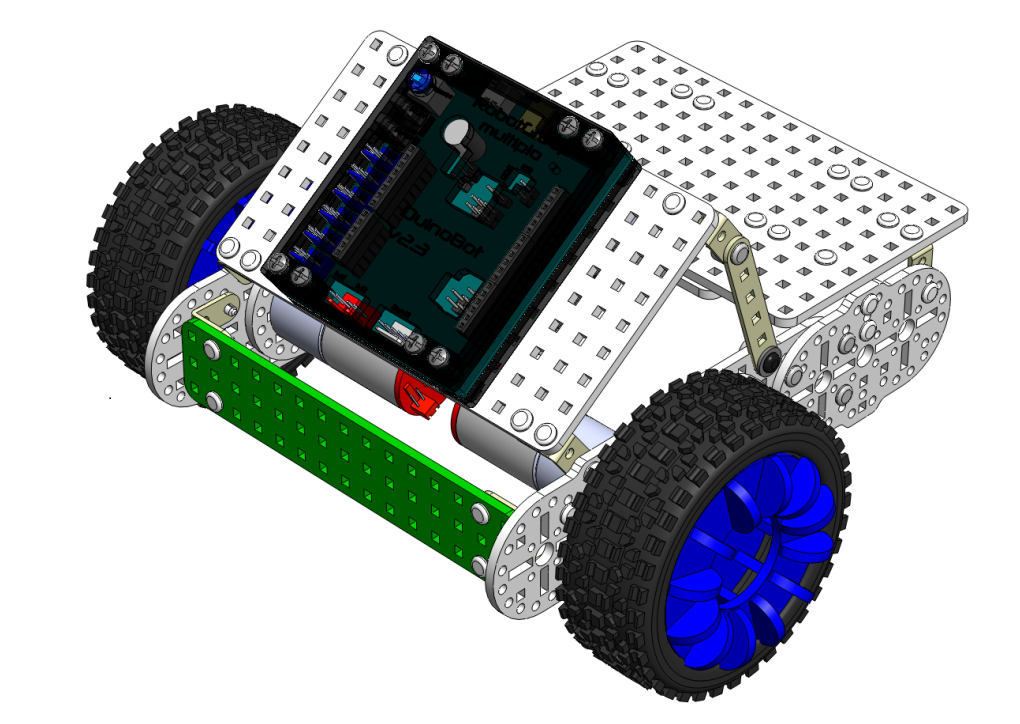
\includegraphics[width=\textwidth]{robot}
         \caption*{ Robot}
         \label{fig:robot}
     \end{subfigure}
     \hfill
     \begin{subfigure}[b]{0.2\textwidth}
         \centering
         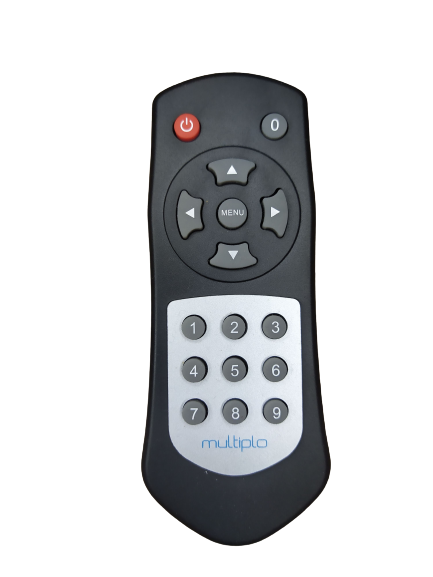
\includegraphics[width=\textwidth]{kumanda_algo}
         \caption*{ Kumanda}
         \label{fig:kumanda}
     \end{subfigure}
     \hfill
     \begin{subfigure}[b]{0.2\textwidth}
         \centering
         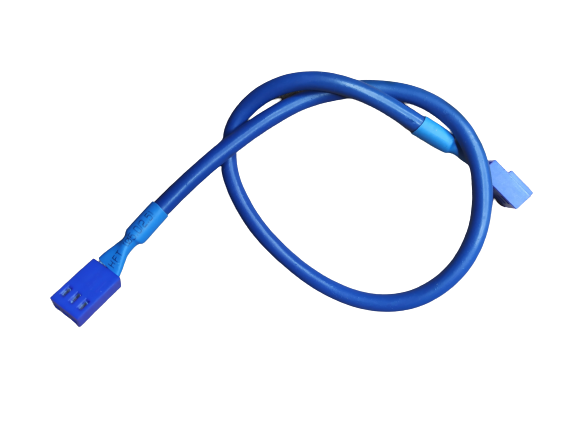
\includegraphics[width=\textwidth]{cable}
         \caption*{ Kablo}
         \label{fig:cable}
     \end{subfigure}
         \hfill
     \begin{subfigure}[b]{0.2\textwidth}
         \centering
         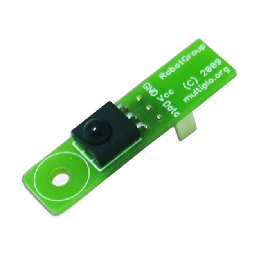
\includegraphics[width=\textwidth]{sensor}
         \caption*{ Sens�r}
         \label{fig:sensor}
     \end{subfigure}
      \caption{�lk uygulamada kulland���m�z malzemeler}
      
\end{figure}

\subsubsection{Engel Alg�lama}
Bu projedeki ikinci uygulamam�z olan robot bir engelle kar��la�t���nda kendi kendine duracakt�r.
Mesafeyi tespit etmek i�in robot, HC-SR04 ultrasonik sens�r� kullan�r. B�ylece bu sens�r her 10 mikrosaniyede bir ultrasonik ses dalgalar� g�nderir ve e�er �n�nde bir engel varsa sens�r yank�y� al�r.

\textbf{Kablolama}\\
Burada size sens�r� robota nas�l ba�layabilece�inizi g�steriyoruz
\begin{figure}[h!]
\centering
  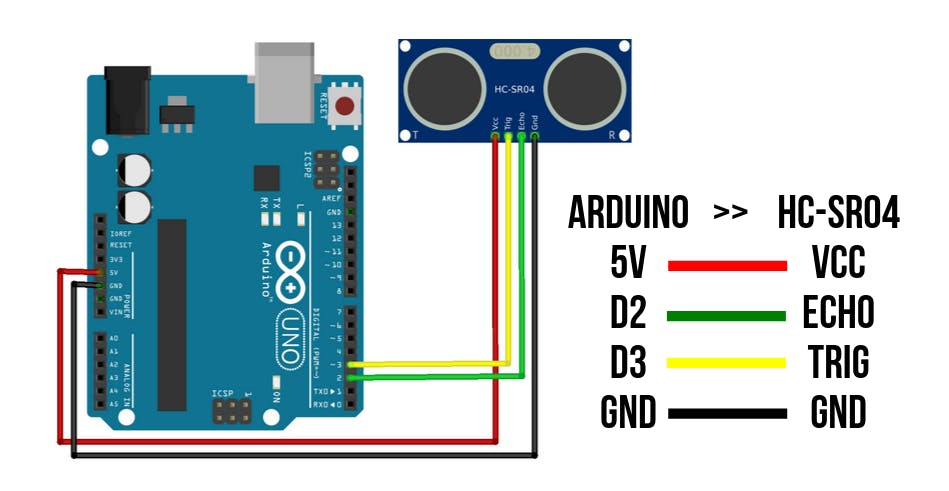
\includegraphics[width=0.9\textwidth]{cablage.jpg}
  \caption{HC-SR04 ultrasonik sens�r� ba�lanmas�}
  \label{fig:cablage}
\end{figure}
\newpage
\textbf{Ak�� Diyagram�}\\
\begin{figure}[h!]
\centering
  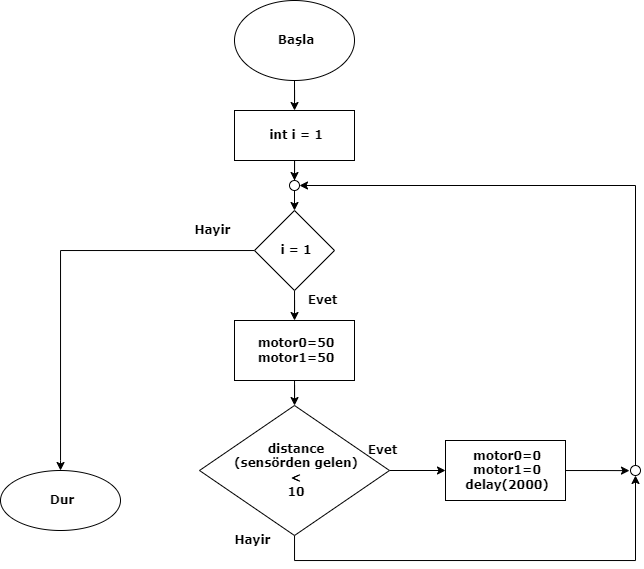
\includegraphics[width=0.9\textwidth]{engel.png}
  \caption{Engel alg�layan robot aki� diyagram�}
  \label{fig:engel}
\end{figure}

Ak�� diyagram� da g�rd���m�z gibi, program� s�rekli �al���r durumda tutmak i�in while d�ng�s� ile ba�latt�k. program otomatik olarak ba�lad���nda robot 50 h�z ile ileri do�ru hareket eder ve ayn� zamanda sens�r sayesinde herhangi bir engel ile aras�ndaki mesafeyi kontrol eder, engele olan mesafe 10'dan az ise robot durur ve sonra her iki saniyede bir engel olup olmad���n� kontrol eder

\newpage
\textbf{Programlama}\\
Kod kismi bakacak olursak
\begin{figure}[h!]
\centering
  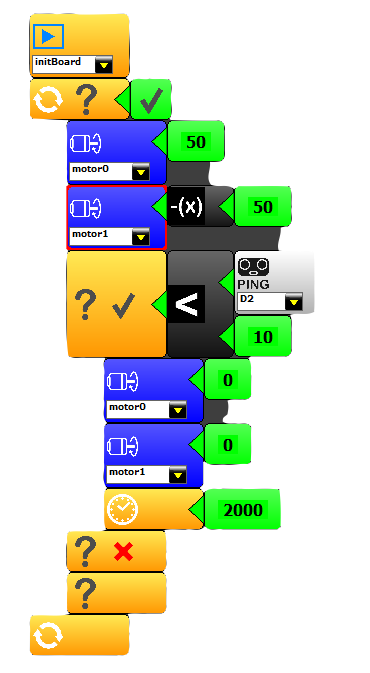
\includegraphics[width=0.7\textwidth]{engel_kod.png}
  \caption{Engel alg�layan robot kodu}
  \label{fig:engel_kod}
\end{figure}


\begin{figure}[h!]
     \centering
     \begin{subfigure}[b]{0.3\textwidth}
         \centering
         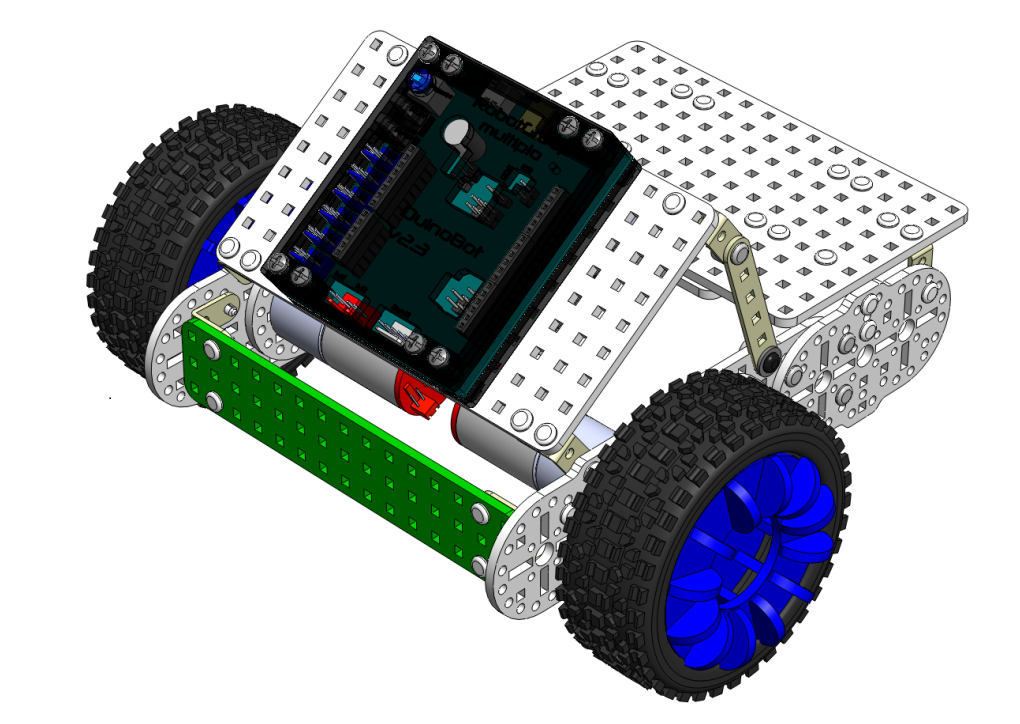
\includegraphics[width=\textwidth]{robot}
         \caption*{ Robot}
         \label{fig:robot}
     \end{subfigure}
     \hfill
     \begin{subfigure}[b]{0.3\textwidth}
         \centering
         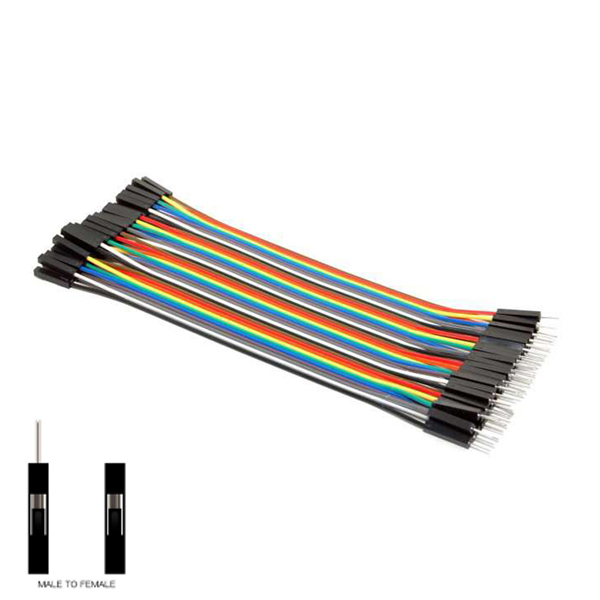
\includegraphics[width=\textwidth]{jumper}
         \caption*{ 4 Adet Erkek-Di�i Jumper}
         \label{fig:kumanda}
     \end{subfigure}
     \hfill
     \begin{subfigure}[b]{0.3\textwidth}
         \centering
         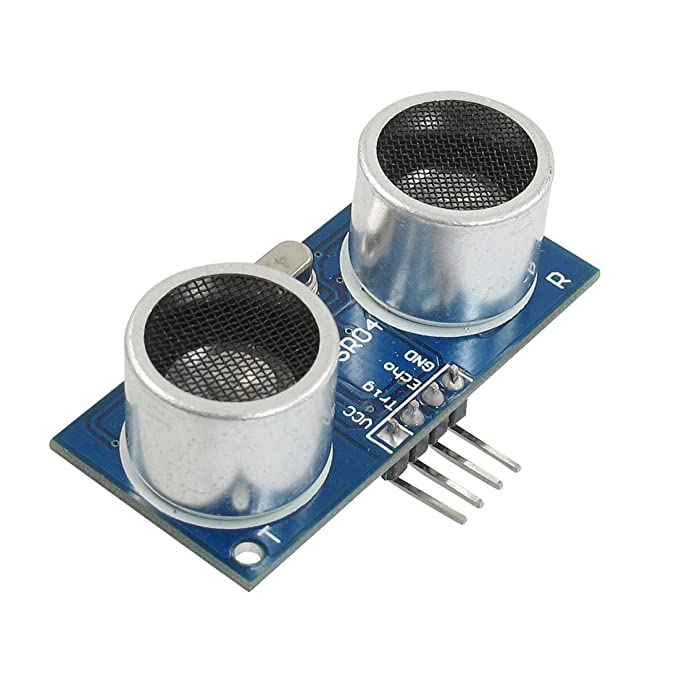
\includegraphics[width=\textwidth]{sens}
         \caption*{ Kablo}
         \label{fig:cable}
     \end{subfigure}
      \caption{�kinci uygulamada kulland���m�z malzemeler}
\end{figure}

\section{SONU�LAR VE �NER�LER}
G�n�m�zde robotik sekt�r� b�y�k bir h�zla b�y�yor. Bu nedenle bu projenin �nemi, ��rencileri bu sekt�re temel bilgilerle tan��t�rarak bu sekt�rde g�ncel olabilmelerini sa�lamakt�r.

Bu projede yapt���m�z uygulamalar �ok esnektir ve ��rencilere de�i�iklik yapma esnekli�i verir ve istedikleri algoritmay� uygulayabilirler.

%\section{Ekler}
\renewcommand{\refname}{KAYNAKLAR}
\addcontentsline{toc}{section}{KAYNAKLAR}
\begin{thebibliography}{99}%kaynak ortam� olu�turmak i�in
%%%%Kaynak Web sayfas�ndan al�nm�� ise%%%%%%%%%%%%%%%%%
\bibitem{k:1} CTAN,\url{http://zelmanov.ptep-online.com/ctan/lshort_turkish.pdf} [Ziyaret Tarihi: 4 Kas�m 2011]\textcolor{red}{---> Kaynak yazar� bilinmeyen yabanc� bir �al��madan al�nm�� ise: }
\bibitem{k:2} Anonymous, 1989, Farm accountancy data network, an
A-Z of methodology, Commission Report of the EC, Brussels, 16-19. 
\bibitem{k:3} \url{http://akgul.bilkent.edu.tr/Yunus/lshort.pdf}
\textcolor{red}{---> Kaynak kongreden al�nm�� ise:}
\bibitem{k:4} Calvalho, M. ve Ludermir, T.B., 2007, Particle Swarm Optimization of Neural Network Architectures and Weights, Seventh International Conference on Hybrid Intelligent Systems, Almanya, 336-339. 
\textcolor{red}{---> Kaynak akt�el dergi ve gazete haberinden al�nm�� ise:} 
\bibitem{k:5} �evkli, M., ve Yenisey, M. M., 2006, At�lye Tipi 
�izelgeleme Problemleri i�in Par�ac�k S�r� Optimizasyonu Y�ntemi, �t�dergisi/d M�hendislik, Cilt 5, Say� 2(1), 58-68.
\textcolor{red}{---> Kaynak akt�el dergi ve gazete haberinden al�nm�� ise:}
\bibitem{k:6} \url{http://kisi.deu.edu.tr/umit.akinci/latexseminer.pdf}\textcolor{red}{---> Kaynak yazar� bilinmeyen ulusal bir �al��madan al�nm�� ise:}
\bibitem{k:7} Anonim, 2006, Tar�m istatistikleri �zeti, D�E Yay�nlar�, No;12, Ankara, 22-23. 
\textcolor{red}{---> Kaynak yazar� bilinmeyen ulusal bir �al��madan al�nm�� ise:}
\end{thebibliography}
\centerline{\textbf{�ZGE�M��}}
\addcontentsline{toc}{section}{�ZGE�M��}
\begin{table}[H]
{
\renewcommand{\arraystretch}{1.5}
\begin{tabular}{l@{\bf :}l}
\multicolumn{2}{l}{\underline{\bf K���SEL B�LG�LER}}\cr
\textbf{Ad� Soyad�}&   IBRAHIM KHALIL ATTEIB YACOUB  \cr
\textbf{Uyru�u}&\; �AD \cr
\textbf{Do�um Yeri ve Tarihi}&\;    03.03.1998\cr
\textbf{Adres}&\;   Bilecik/T�rkiye   \cr
\multicolumn{1}{l}{}&      \cr
\textbf{Telefon}&\;  5433044170   \cr
\textbf{e-mail}&\; ibrahimalkhalilatteib@gmail.com  \cr
\multicolumn{1}{l}{}&\cr
\multicolumn{2}{l}{\underline{\bf E��T�M DURUMU}}\cr
\textbf{Lisans ��renimi}&\; B�E� Bilgisayar M�hendisli�i B�l�m�\cr
\textbf{Bitirme Y�l�}&\;  2023  \cr
\textbf{Lise}& \; Kuveyt merkez lisesi   \cr
\multicolumn{1}{l}{}&\cr
\multicolumn{2}{l}{\underline{\bf �� DENEY�MLER�}}\cr
\textbf{Y�l}&\;  -   \cr
\textbf{Kurum}& \;  -  \cr
\textbf{Stajlar}&\;  -   \cr
\multicolumn{1}{l}{}&\cr
\multicolumn{2}{l}{\underline{\bf �LG� ALANLARI:}}Yapay Zeka, Web Uygulama (Laravel)\cr
\multicolumn{1}{l}{}&\cr
\multicolumn{2}{l}{\underline{\bf YABANCI D�LLER:}}Fransizca, Arap�a, �ngilizce(ba�lang��)\cr
\multicolumn{1}{l}{}&\cr


\end{tabular}}
\end{table}
\shorthandon{=}
\end{document}
%%%%%%%%%%%%%%%%%%%%%%%%%%%B�TT�%%%%%%%%%%%%%%%%%%%%%%%%%%%%%%%%%%%%%%%%%%%%%
